%package list
\documentclass{article}
\usepackage[top=3cm, bottom=3cm, outer=3cm, inner=3cm]{geometry}
\usepackage{multicol}
\usepackage{graphicx}
\usepackage{url}
%\usepackage{cite}
\usepackage{hyperref}
\usepackage{array}
%\usepackage{multicol}
\newcolumntype{x}[1]{>{\centering\arraybackslash\hspace{0pt}}p{#1}}
\usepackage{natbib}
\usepackage{pdfpages}
\usepackage{multirow}
\usepackage[normalem]{ulem}
\useunder{\uline}{\ul}{}
\usepackage{svg}
\usepackage{xcolor}
\usepackage{listings}
\lstdefinestyle{ascii-tree}{
    literate={├}{|}1 {─}{--}1 {└}{+}1 
  }
\lstset{basicstyle=\ttfamily,
  showstringspaces=false,
  commentstyle=\color{red},
  keywordstyle=\color{blue}
}
%\usepackage{booktabs}
\usepackage{caption}
\usepackage{subcaption}
\usepackage{float}
\usepackage{array}

\newcolumntype{M}[1]{>{\centering\arraybackslash}m{#1}}
\newcolumntype{N}{@{}m{0pt}@{}}


%%%%%%%%%%%%%%%%%%%%%%%%%%%%%%%%%%%%%%%%%%%%%%%%%%%%%%%%%%%%%%%%%%%%%%%%%%%%
%%%%%%%%%%%%%%%%%%%%%%%%%%%%%%%%%%%%%%%%%%%%%%%%%%%%%%%%%%%%%%%%%%%%%%%%%%%%
\newcommand{\itemEmail}{fgarambel@unsa.edu.pe}
\newcommand{\itemStudent}{Fernando Miguel Garambel Marín}
\newcommand{\itemCourse}{Laboratorio de Programación Web 2}
\newcommand{\itemCourseCode}{1701212}
\newcommand{\itemSemester}{III}
\newcommand{\itemUniversity}{Universidad Nacional de San Agustín de Arequipa}
\newcommand{\itemFaculty}{Facultad de Ingeniería de Producción y Servicios}
\newcommand{\itemDepartment}{Departamento Académico de Ingeniería de Sistemas e Informática}
\newcommand{\itemSchool}{Escuela Profesional de Ingeniería de Sistemas}
\newcommand{\itemAcademic}{2024 - A}
\newcommand{\itemInput}{Del 9 de abril 2024}
\newcommand{\itemOutput}{Al 25 de mayo 2024}
\newcommand{\itemPracticeNumber}{05}
\newcommand{\itemTheme}{Python}
%%%%%%%%%%%%%%%%%%%%%%%%%%%%%%%%%%%%%%%%%%%%%%%%%%%%%%%%%%%%%%%%%%%%%%%%%%%%
%%%%%%%%%%%%%%%%%%%%%%%%%%%%%%%%%%%%%%%%%%%%%%%%%%%%%%%%%%%%%%%%%%%%%%%%%%%%

\usepackage[english,spanish]{babel}
\usepackage[utf8]{inputenc}
\AtBeginDocument{\selectlanguage{spanish}}
\renewcommand{\figurename}{Figura}
\renewcommand{\refname}{Referencias}
\renewcommand{\tablename}{Tabla} %esto no funciona cuando se usa babel
\AtBeginDocument{%
	\renewcommand\tablename{Tabla}
}

\usepackage{fancyhdr}
\pagestyle{fancy}
\fancyhf{}
\setlength{\headheight}{30pt}
\renewcommand{\headrulewidth}{1pt}
\renewcommand{\footrulewidth}{1pt}
\fancyhead[L]{\raisebox{-0.2\height}{
\includegraphics[width=3cm]{img/logo_episunsa.png}}}
\fancyhead[C]{\fontsize{7}{7}\selectfont	\itemUniversity \\ \itemFaculty \\ \itemDepartment \\ \itemSchool \\ \textbf{\itemCourse}}
\fancyhead[R]{\raisebox{-0.2\height}{
\includegraphics[width=1.2cm]{img/logo_abet}}}
\fancyfoot[L]{Fernando Garambel}
\fancyfoot[C]{\itemCourse}
\fancyfoot[R]{Página \thepage}

% para el codigo fuente
\usepackage{listings}
\usepackage{color, colortbl}
\definecolor{dkgreen}{rgb}{0,0.6,0}
\definecolor{gray}{rgb}{0.5,0.5,0.5}
\definecolor{mauve}{rgb}{0.58,0,0.82}
\definecolor{codebackground}{rgb}{0.95, 0.95, 0.92}
\definecolor{tablebackground}{rgb}{0.8, 0, 0}

\lstset{frame=tb,
	language=bash,
	aboveskip=3mm,
	belowskip=3mm,
	showstringspaces=false,
	columns=flexible,
	basicstyle={\small\ttfamily},
	numbers=none,
	numberstyle=\tiny\color{gray},
	keywordstyle=\color{blue},
	commentstyle=\color{dkgreen},
	stringstyle=\color{mauve},
	breaklines=true,
	breakatwhitespace=true,
	tabsize=3,
	backgroundcolor= \color{codebackground},
}

\begin{document}
	
	\vspace*{10px}
	
	\begin{center}	
		\fontsize{17}{17} \textbf{ Informe de Laboratorio \itemPracticeNumber}
	\end{center}
	\centerline{\textbf{\Large Tema: \itemTheme}}
	%\vspace*{0.5cm}	

	\begin{flushright}
		\begin{tabular}{|M{2.5cm}|N|}
			\hline 
			\rowcolor{tablebackground}
			\color{white} \textbf{Nota}  \\
			\hline 
			     \\[30pt]
			\hline 			
		\end{tabular}
	\end{flushright}	

	\begin{table}[H]
		\begin{tabular}{|x{4.7cm}|x{4.8cm}|x{4.8cm}|}
			\hline 
			\rowcolor{tablebackground}
			\color{white} \textbf{Estudiante} & \color{white}\textbf{Escuela}  & \color{white}\textbf{Asignatura}   \\
			\hline 
			{\itemStudent \par \itemEmail} & \itemSchool & {\itemCourse \par Semestre: \itemSemester \par Código: \itemCourseCode}     \\
			\hline 			
		\end{tabular}
	\end{table}		
	
	\begin{table}[H]
		\begin{tabular}{|x{4.7cm}|x{4.8cm}|x{4.8cm}|}
			\hline 
			\rowcolor{tablebackground}
			\color{white}\textbf{Laboratorio} & \color{white}\textbf{Tema}  & \color{white}\textbf{Duración}   \\
			\hline 
			\itemPracticeNumber & \itemTheme & 04 horas   \\
			\hline 
		\end{tabular}
	\end{table}
	
	\begin{table}[H]
		\begin{tabular}{|x{4.7cm}|x{4.8cm}|x{4.8cm}|}
			\hline 
			\rowcolor{tablebackground}
			\color{white}\textbf{Semestre académico} & \color{white}\textbf{Fecha de inicio}  & \color{white}\textbf{Fecha de entrega}   \\
			\hline 
			\itemAcademic & \itemInput &  \itemOutput  \\
			\hline 
		\end{tabular}
	\end{table}
	
\section{Actividades}
	\begin{itemize}		
		\item Practicar los principios de de programación usando Python
		\item Mostrar un ejemplo de separación de intereses en clases: el modelo (lista de strings) de su vista (dibujo de gráficos).
	\end{itemize}

\section{Ejercicios Propuestos}
	\begin{itemize}		
		\item En esta tarea, individualmente usted pondrá en práctica sus conocimientos de programación en Python para dibujar un tablero de Ajedrez. La parte gráfica ya está programada, usted sólo tendrá que concentrarse en las estructuras de datos subyacentes.
		\item Con el código proporcionado usted dispondrá de varios objetos de tipo Picture para poder realizar su tarea:
		\begin{figure}[H]
		\centering
		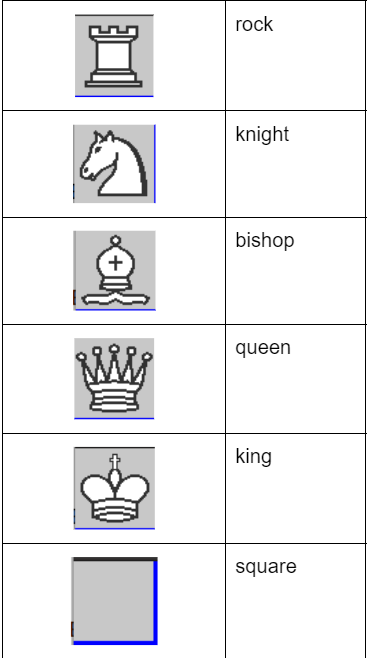
\includegraphics[width=0.7\textwidth,keepaspectratio]{img/Piezas.png}
		%\includesvg{img/automata.svg}
		%\label{img:mot2}
		%\caption{Product backlog.}
	\end{figure}
		\item Estos objetos estarán disponibles importando la biblioteca: chessPictures y estarán internamente representados con arreglos de strings que podrá revisar en el archivo pieces.py
		\item La clase Picture tiene un sólo atributo: el arreglo de strings img, el cual contendrá la representación en caracteres de la figura que se desea dibujar. 
La clase Picture ya cuenta con una función implementada, no debe modificarla, pero si puede usarla para implementar sus otras funciones: invColor: recibe un color como un carácter de texto y devuelve su color negativo, también como texto, deberá revisar el archivo colors.py para conocer los valores negativos de cada carácter.
		\item La clase Picture contará además con varios métodos que usted deberá implementar:
		\item verticalMirror: Devuelve el espejo vertical de la imagen
		\item horizontalMirror: Devuelve el espejo horizontal de la imagen
		\item negative: Devuelve un negativo de la imagen
		\item join: Devuelve una nueva figura poniendo la figura del argumento al lado derecho de la figura actual
		\item up: Devuelve una nueva figura poniendo la figura recibida como argumento, encima de la figura actual
		\item under: Devuelve una nueva figura poniendo la figura recibida como argumento, sobre la figura actual
		\item horizontalRepeat, Devuelve una nueva figura repitiendo la figura actual al costado la cantidad de veces que indique el valor de n
		\item verticalRepeat Devuelve una nueva figura repitiendo la figura actual debajo, la cantidad de veces que indique el valor de n
		\item Tenga en cuenta que para implementar todos estos métodos, sólo deberá trabajar sobre la representación interna de un Picture, es decir su atributo img.
		\item Para dibujar una objeto Picture bastará importar el método draw de la biblioteca interpreter y usarlo de la siguiente manera:
		\item from chessPictures import *
 from interpreter import draw
draw(rock)
		\item Considerar el repositorio:
		\item \url{https://github.com/rescobedoq/pw2/tree/main/labs/lab04/Tarea-del-Ajedrez}
	\end{itemize}
	\section{Equipos, materiales y temas utilizados}
	\begin{itemize}
		\item Sistema operativo de 64 bits, procesador basado en x64.
		\item Latex. 
		\item git version 2.41.0.windows.1
		\item Cuenta en GitHub con el correo institucional.
	\end{itemize}
	\section{URL Github, Video}
	\begin{itemize}
		\item URL del Repositorio GitHub para clonar o recuperar.
		\item \url{https://github.com/FernandoGarambelM/Python-Ajedrez.git}
		\item URL para el video flipgrid.
		\item \url{https://flip.com/s/iFLsg1o2c_wh}	
	\end{itemize}
	\clearpage
	\section{Ejercicios}
	\begin{itemize}
		\item Para resolver los siguientes ejercicios sólo está permitido usar ciclos, condicionales, definición de listas por comprensión, sublistas, map, join, (+), lambda, zip, append, pop, range.
		\item Implemente los métodos de la clase Picture. Se recomienda que implemente la clase picture por etapas, probando realizar los dibujos que se muestran en la siguiente preguntas.
		\item Usando únicamente los métodos de los objetos de la clase Picture dibuje las siguientes figuras (invoque a draw):
	\end{itemize}
	\begin{figure}[H]
		\centering
		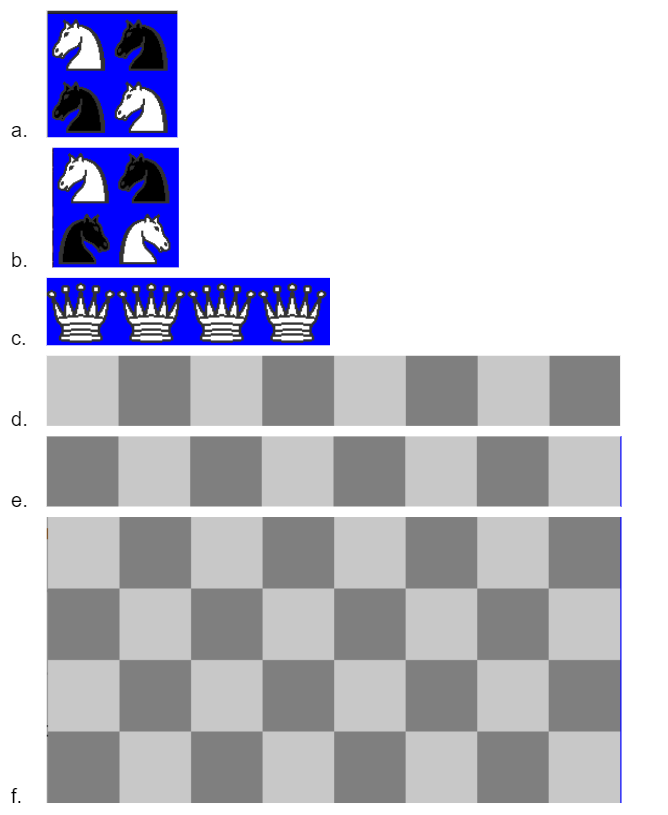
\includegraphics[width=0.7\textwidth,keepaspectratio]{img/Ejercicios.png}
		%\includesvg{img/automata.svg}
		%\label{img:mot2}
		%\caption{Product backlog.}
	\end{figure}
	\begin{figure}[H]
		\centering
		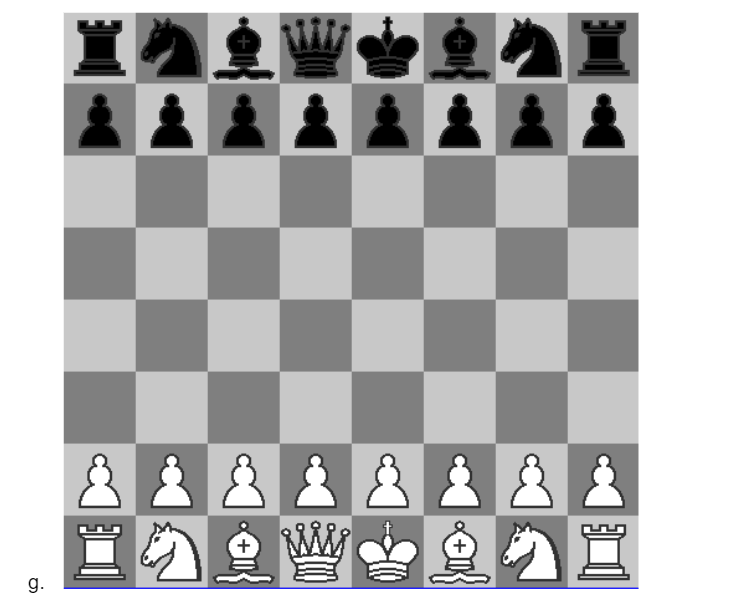
\includegraphics[width=0.7\textwidth,keepaspectratio]{img/Ejercicio.png}
		%\includesvg{img/automata.svg}
		%\label{img:mot2}
		%\caption{Product backlog.}
	\end{figure}
\section{Implementación de funciones de Picture}
	\begin{lstlisting}[language=Python,caption={Función verticalMirror(self)}][H]
def verticalMirror(self):
    vertical = []
    for value in self.img:
      vertical.append(value[::-1])
    return Picture(vertical)
	\end{lstlisting}
	\begin{itemize}
		\item Devuelve el espejo vertical de la imagen 
	\end{itemize}
	\begin{lstlisting}[language=Python,caption={Función horizontalMirror(self)}][H]
def horizontalMirror(self):
    horizontal = []
    for value in self.img[::-1]:
      horizontal.append(value)
    return Picture(horizontal)
	\end{lstlisting}
	\begin{itemize}
		\item Devuelve el espejo horizontal de la imagen
	\end{itemize}
	\begin{lstlisting}[language=Python,caption={Función negative(self)}][H]
def negative(self):
    negative = []
    for value in self.img:
      negative.append([self._invColor(color) for color in value])
    return Picture(negative)
	\end{lstlisting}
	\begin{itemize}
		\item Devuelve un negativo de la imagen 
	\end{itemize}
	\begin{lstlisting}[language=Python,caption={Función join(self, p)}][H]
def join(self, p):
    joinedImg = []
    for i in range(len(self.img)):
        joinedRow = "".join(self.img[i]) + "".join(p.img[i])
        joinedImg.append(joinedRow)
    return Picture(joinedImg)
	\end{lstlisting}
	\begin{itemize}
		\item Devuelve una nueva figura poniendo la figura del argumento al lado derecho de la figura actual
	\end{itemize}
	\begin{lstlisting}[language=Python,caption={Función up(self, p)}][H]
def up(self, p):
    uping = []
    for value in self.img:
      uping.append(value)
    for value in p.img:
      uping.append(value)
    return Picture(uping)
	\end{lstlisting}
	\begin{itemize}
		\item Devuelve una nueva figura poniendo la figura actual por encima de la del argumento
	\end{itemize}
	\begin{lstlisting}[language=Python,caption={Función VerticalMirror()}][H]
def verticalMirror(self):
    vertical = []
    for value in self.img:
      vertical.append(value[::-1])
    return Picture(vertical)
	\end{lstlisting}
	\begin{itemize}
		\item Devuelve el espejo vertical de la imagen 
	\end{itemize}



	\lstinputlisting[language=Python, caption={Código de Picture},numbers=left,]{src/picture.py}
\section{Referencias}
\begin{itemize}			
	\item \url{https://www.w3schools.com/python/python_reference.asp}
	\item\url{https://docs.python.org/3/tutorial/ complex and powerful}
\end{itemize}	
	
%\clearpage
%\bibliographystyle{apalike}
%\bibliographystyle{IEEEtranN}
%\bibliography{bibliography}
			
\end{document}